% !BIB program = biber
%\documentclass[xcolor=dvipsnames, aspectratio=169, handout]{beamer}
\documentclass[xcolor=dvipsnames, aspectratio=169]{beamer}
\usetheme{Madrid}
%\usetheme{Rochester}
\usepackage{transparent}


\usepackage{amsthm}
%\usepackage{fontspec}
\usepackage{amssymb}

% \usepackage{graphicx}
%\usepackage{cite}
\usepackage{caption}
\usepackage{float}
% \usepackage{fancyhdr}
%\usepackage{enumitem}
\usepackage{bbm}
\definecolor{Blue}{rgb}{0,0,1}
\definecolor{Red}{rgb}{1,0,0}
%\usepackage{subfig}
% \usepackage[colorlinks=true,linkcolor=Red,urlcolor=Blue,citecolor=Red]{hyperref}
% \pagestyle{fancy}
%\usepackage[top=3cm, bottom=3cm, left=3cm, right=3cm]{geometry}

\usepackage{perpage}
\usepackage{hyperref}
\usepackage{epsfig}
%\usepackage[top=2cm, bottom=2cm, outer=0cm, inner=0cm]{geometry}



\newtheorem{remark}[theorem]{Remark}
\newtheorem{algg}[theorem]{Algorithm}
 \usepackage{tikz}
\usetikzlibrary{
	arrows,
	mindmap,
	trees,
	shadows,
	graphs,
	graphs.standard,
	decorations.markings,
	intersections,
	calc,
	backgrounds,
	chains,fit,shapes
}

%
%
\def\HG{{\mathcal G}}
\def\gplus#1{\mathop{+\!\!_{_#1}}}
\def\gtimes#1{\mathop{\times\!\!_{_#1}}}
\def\hgn{\text{\rm HG}}
\def\cnst#1{\star #1}
\usepackage{xargs}
\usepackage[colorinlistoftodos,prependcaption,textsize=small]{todonotes}
\newcommandx{\unsure}[2][1=]{\todo[linecolor=red,backgroundcolor=red!25,bordercolor=red,#1]{#2}}
\newcommandx{\change}[2][1=]{\todo[linecolor=blue,backgroundcolor=blue!25,bordercolor=blue,#1]{#2}}
\newcommandx{\info}[2][1=]{\todo[linecolor=OliveGreen,backgroundcolor=OliveGreen!25,bordercolor=OliveGreen,#1]{#2}}
\newcommandx{\improvement}[2][1=]{\todo[linecolor=Plum,backgroundcolor=Plum!25,bordercolor=Plum,#1]{#2}}
\newcommandx{\thiswillnotshow}[2][1=]{\todo[disable,#1]{#2}}
%

\tikzstyle{win_nodes}=[circle, draw=black, inner sep=1.5, fill=black]
\tikzstyle{win_edges}=[draw=black, thick]
\tikzstyle{lose_nodes}=[circle, draw=black, inner sep=1.5, fill=black]
\tikzstyle{lose_edges}=[draw=black, thick]

\definecolor{lgreen}{RGB}{180, 180, 180}
\tikzstyle{vecArrow} = [thick, decoration={markings,mark=at position
1 with {\arrow[semithick]{open triangle 60}}},
double distance=1.4pt, shorten >= 5.5pt,
preaction = {decorate},
postaction = {draw,line width=1.4pt, white,shorten >= 4.5pt}]
\tikzstyle{innerWhite} = [semithick, white,line width=1.4pt, shorten >= 4.5pt]

\usefonttheme{structurebold}
\usefonttheme[onlymath]{serif}

\definecolor{Mycolor2}{HTML}{174D51}
\definecolor{tit}{HTML}{8c7023}
%\usecolortheme{beaver}

%\usecolortheme[named=Mycolor2]{structure}
\setbeamercolor{title}{fg=tit,bg=}
\setbeamersize{text margin left=20mm,text margin right=20mm}
%
\setbeamercolor{palette primary}{bg=Mycolor2,fg=white} % banner and third sub banne
\setbeamercolor{palette secondary}{bg=Mycolor2,fg=white}
\setbeamercolor{palette tertiary}{bg=Mycolor2,fg=white}
\setbeamercolor{palette quaternary}{bg=red,fg=white}
%\BeforeBeginEnvironment{definition}{%
%	\setbeamercolor{block title}{fg=black,bg=pink!50!white}
%	\setbeamercolor{block body}{fg=pink, bg=pink!30!white}
%}
%\AfterEndEnvironment{definition}{
%	\setbeamercolor{block title}{use=structure,fg=structure.fg,bg=structure.fg!20!bg}
%	\setbeamercolor{block body}{parent=normal text,use=block title,bg=block title.bg!50!bg, fg=black}
%}

\setbeamercolor{block title example}{use=example text,fg=example text.fg,bg=example text.fg!20!bg}
\setbeamercolor{block body example}{parent=normal text,use=block title example,bg=block title example.bg!50!bg}

%\setbeamercolor{block title definition}{use=example text,fg=example text.fg,bg=example text.fg!20!bg}
%\setbeamercolor{block body definition}{parent=normal text,use=block title example,bg=block title example.bg!50!bg}

%\setbeamercolor{structure}{fg=black} % itemize, enumerate, etc
\setbeamercolor{section in toc}{fg=black} % TOC sections
\definecolor{UBCgrey}{rgb}{0.3686, 0.5255, 0.6235} % UBC Grey (secondary)

% Override palette coloring with secondary
\setbeamercolor{subsection in head/foot}{bg=black,fg=white}
\setbeamertemplate{caption}[numbered]

\usepackage[utf8]{inputenc}
\usepackage[T1]{fontenc}    % use 8-bit T1 fonts
\usepackage{url}            % simple URL typesetting
\usepackage{booktabs}       % professional-quality tables
\usepackage{amsfonts}       % blackboard math symbols
\usepackage{nicefrac}       % compact symbols for 1/2, etc.
\usepackage{microtype}      % microtypography
\usepackage{mathtools}
\usepackage{multicol}
\usepackage{comment}
\usepackage{forest}
\usepackage[linesnumbered, ruled]{algorithm2e}
\usepackage{algorithmic}
\usepackage[dvipsnames]{xcolor}
\usepackage{colortbl}
\usepackage{graphicx}
\usepackage{diagbox}
\usetikzlibrary{fadings}
\usepackage{caption}
\usepackage{subcaption}
% \captionsetup[subfigure]{labelsep=space}
\usepackage{amsmath}
\usepackage{dsfont}
\usepackage{stmaryrd}
\bibliographystyle{plainnat}
%\bibliographystyle{ieeetr}
%\usepackage[round]{natbib}   % omit 'round' option if you prefer square brackets
\usepackage[style=authoryear,backend=bibtex]{biblatex}
\addbibresource{refs.bib}

\renewcommand{\footnotesize}{\tiny}
\newcommand{\mathbi}[1]{\boldsymbol{#1}}
\newtheorem{proposition}{Proposition}
\newcommand{\set}[1]{\left\{ #1 \right\}}
\newcommand{\seq}[1]{\left< #1 \right>}
\newcommand{\ceil}[1]{\left\lceil{#1}\right\rceil}
\newcommand{\floor}[1]{\left\lfloor{#1}\right\rfloor}
\newcommand{\card}[1]{\left|{#1}\right|}
\newcommand{\setcomp}[1]{\overline{#1}}

%------------------------------------------------------------
%This block of code defines the information to appear in the
%Title page
%\addtobeamertemplate{frametitle}{}{
%	\raisebox{0.1cm}[0pt][0pt]{\hfill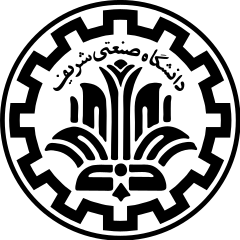
\includegraphics[height=1cm]{images/sharif}}
%	\hspace{0.2cm}\vspace{-1.1cm}
%	}
	\logo{
		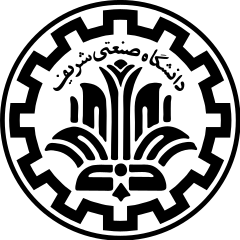
\includegraphics[width=1cm]{images/sharif}
}
%\setbeamertemplate{headline}{\hfill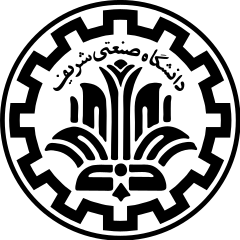
\includegraphics[width=1cm]{images/sharif}\hspace{0.2cm}\vspace{-1.1cm}}
\title[On Pliable Index Coding] %optional
{\\\textbf{On Pliable Index Coding}}

\subtitle{}

\author[Hossein Mahdavipour] % (optional)
{Hossein Mahdavipour\\
	Supervisor: Javad B. Ebrahimi}


\institute[SUT] % (optional)
{
	\small MSc Thesis \\
	Department of Mathematical Sciences \\
	Sharif University of Technology % Your institution for the title page
}
\newcommand{\rdss}{\mathrm{RDSS}}
\newcommand{\indx}{\mathrm{INDEX}}


%End of title page configuration block
%------------------------------------------------------------



%------------------------------------------------------------
%The next block of commands puts the table of contents at the 
%beginning of each section and highlights the current section:

\AtBeginSection[]
{
  \begin{frame}
    \frametitle{Table of Contents}
    \tableofcontents[currentsection]
  \end{frame}
}
%------------------------------------------------------------


\begin{document}

% The next statement creates the title page.
\setbeamertemplate{background canvas}{
	
\includegraphics[height=\paperheight]{images/Background}
	}

\begin{frame}[plain]
	\tikz[remember picture,overlay] \node[opacity=1,inner sep=0pt] at ($(current page.north)+(0,-1cm)$){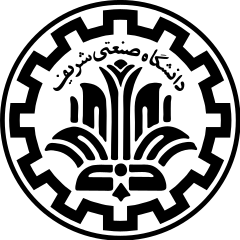
\includegraphics[height=0.15\paperheight]{images/sharif}};
	\vfill
\titlepage
\end{frame}


\setbeamertemplate{background canvas}{
	\transparent{0.2}
\includegraphics[width=\paperwidth,height=\paperheight]{images/Background}
}


%---------------------------------------------------------
%This block of code is for the table of contents after
%the title page
\begin{frame}
\frametitle{Table of Contents}
\tableofcontents
\end{frame}

%------------------------------------------------
\section{Introduction}
%------------------------------------------------

\begin{frame}
	\centering
	\Huge
	Introduction
\end{frame}
\subsection{Real World Example}
\begin{frame}{Problem}
	\centering
	\begin{tikzpicture}[->, >=stealth, auto, semithick]
		% Set the positions of the nodes
		\alt<1,2,3,4>{
			\node[circle, draw=blue, fill=blue!20, inner sep=0pt] (P1) at (0,-2) {
				
\includegraphics[width=0.07\linewidth]{img/hosseinmp76}
			};	
		}{
			\node[circle, draw=blue, fill=blue!20, inner sep=0pt] (P1) at (-3,-2) {
				
\includegraphics[width=0.07\linewidth]{img/hosseinmp76}
			};
		}
		\alt<5->{\node[circle, draw=blue, fill=blue!20, inner sep=0pt] (P2) at (3,-2) {
				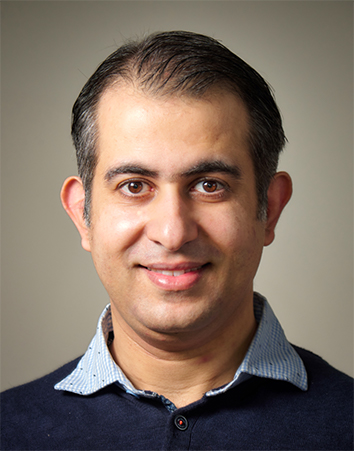
\includegraphics[width=0.06\linewidth]{img/javad}};
		}{}
		
		\alt<5->{\node[above] at (0,-3.5) {people};}{}
		
		\alt<2-5>{
			\node[circle, draw=red, fill=red!20, inner sep=0pt] (M1) at (0,0) {
				
\includegraphics[width=0.07\linewidth]{img/fox}
				
			};

		}{}
		\alt<6->{
			\node[circle, draw=red, fill=red!20, inner sep=0pt] (M1) at (-6,0) {
				
\includegraphics[width=0.1\linewidth]{img/45140_satellite_icon}
				
			};
		}{}
		\alt<3->{
			\node[circle, draw=green, fill=green!20, inner sep=0pt] (N1) at (-3,2) {
				
\includegraphics[width=0.1\linewidth]{img/fox5}
				
				
			};
			\node[circle, draw=green, fill=green!20, inner sep=0pt] (N2) at (0,2) {
				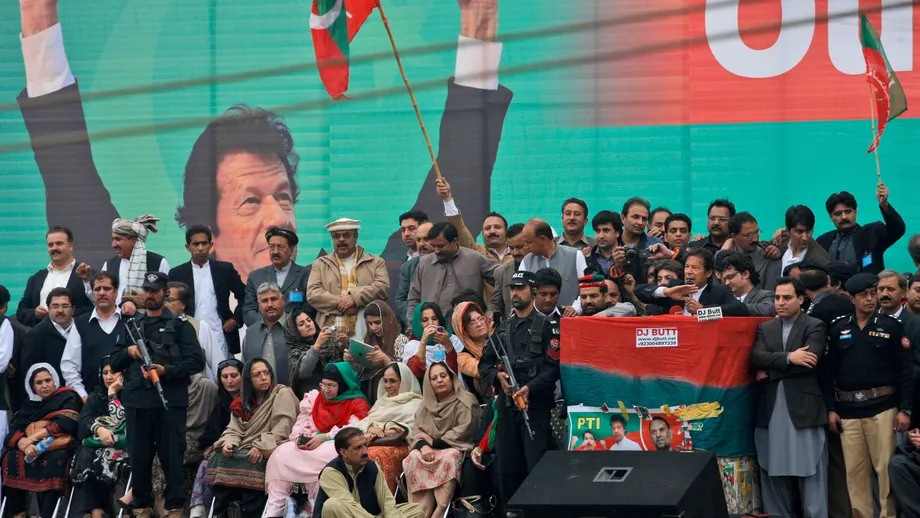
\includegraphics[width=0.1\linewidth]{img/fox3}
				
			};
			\node[circle, draw=green, fill=green!20, inner sep=0pt] (N3) at (3,2) {
				
\includegraphics[width=0.1\linewidth]{img/fox4}
				
			};
			\node[below] at (0,3.5) {news };
		}{}
		
		\alt<2-5>{
			% Draw the edges
			\draw[-] (P1) -- (M1);
		}{}
		\alt<3-5>{
			% Draw the edges
			\draw[-]  (M1) -- (N1) ;
			\draw[-]  (M1) -- (N2) ;
			\draw[-]  (M1) -- (N3) ;
		}{}
		\alt<5>{
			% Draw the edges
			\draw[-]  (P2) -- (M1);
		}{}
		\alt<4->{
			% Draw the edges
			\draw[->, color=red] (P1) -- (N1);
		}{}
		\alt<5->{
			% Draw the edges
			\draw[->, color=red] (P2) -- (N2);
			\draw[->, color=red] (P2) -- (N3);
		}{}
	\end{tikzpicture}
\end{frame}

\subsection{Aapplications}
\begin{frame}{Aapplications}
	\begin{columns}[c] % The "c" option specifies centered vertical alignment while the "t" option is used for top vertical alignment
		\column{.5\textwidth} % Left column and width
		\begin{itemize}
			\item<1-> distributed storage: \textcite{arya}
			\item<2-> Machine learning: \textcite{datashuff}
		\end{itemize}
		\column{.7\textwidth} % Right column and width			
		\alt<1>{\begin{figure}
				\centering
				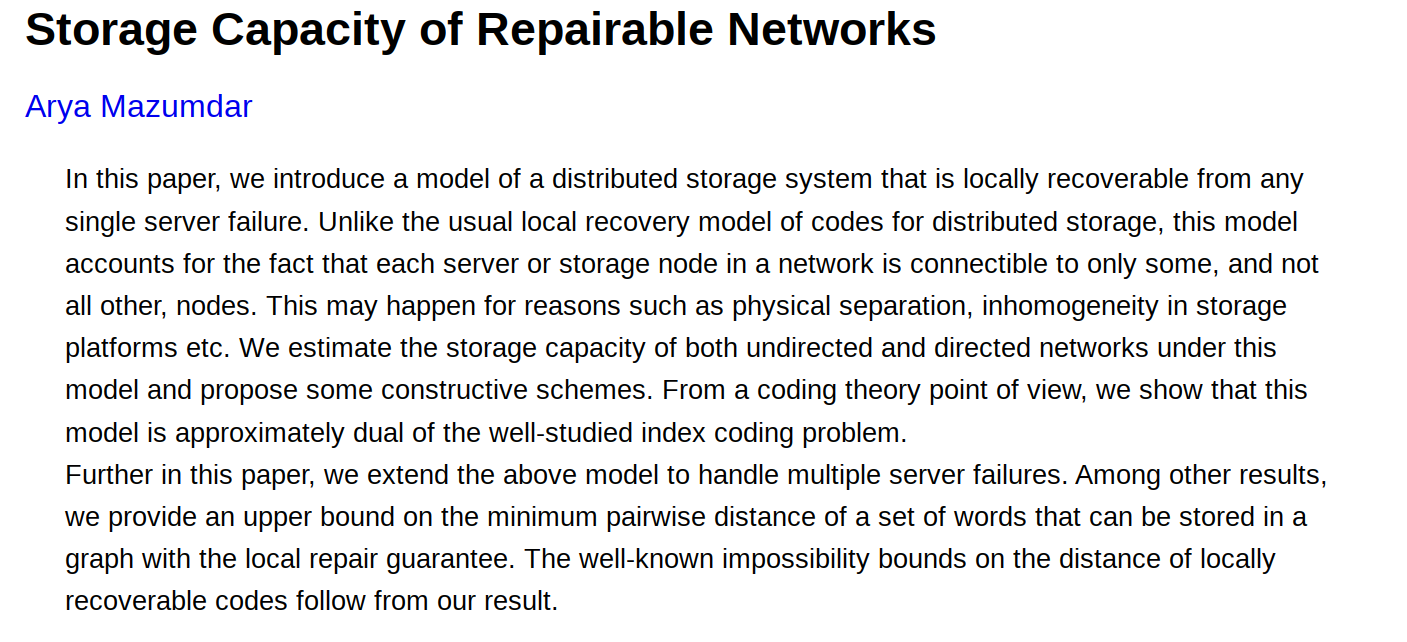
\includegraphics[width=.7\linewidth]{img/arya}
		\end{figure}}{}
		\alt<2>{\begin{figure}
				\centering
				\includegraphics[width=.7\linewidth]{"img/datashuffel"}
				%	\caption{}
				%	\label{fig:dynamic-index-coding-for-wireless-broadcastnetworks}
		\end{figure}}{}

	\end{columns}
\end{frame}

\subsection{PICOD Informal Difination}
\begin{frame}{PICOD}
	\begin{columns}[c] % The "c" option specifies centered vertical alignment while the "t" option is used for top vertical alignment
		
		\column{.7\textwidth} % Left column and width
		\begin{itemize}
			\item<1-> Introduced by \textcite{pliablefirstpaper} item as a special case of general index coding introduced by \textcite{firstpaper}
			\item<2-> One broadcaster, m clients, n messages.
			\item<3-> Clients are pliable, seeking any not-known message
			\item<4-> Find the minimum needed transmission
			\item<5-> NP-hard
		\end{itemize}
		\column{.4\textwidth} % Right column and width
		%			\includegraphics[width=0.7\linewidth]{img/screenshot005}
		\alt<1>{}{
			\begin{figure}
				\centering
				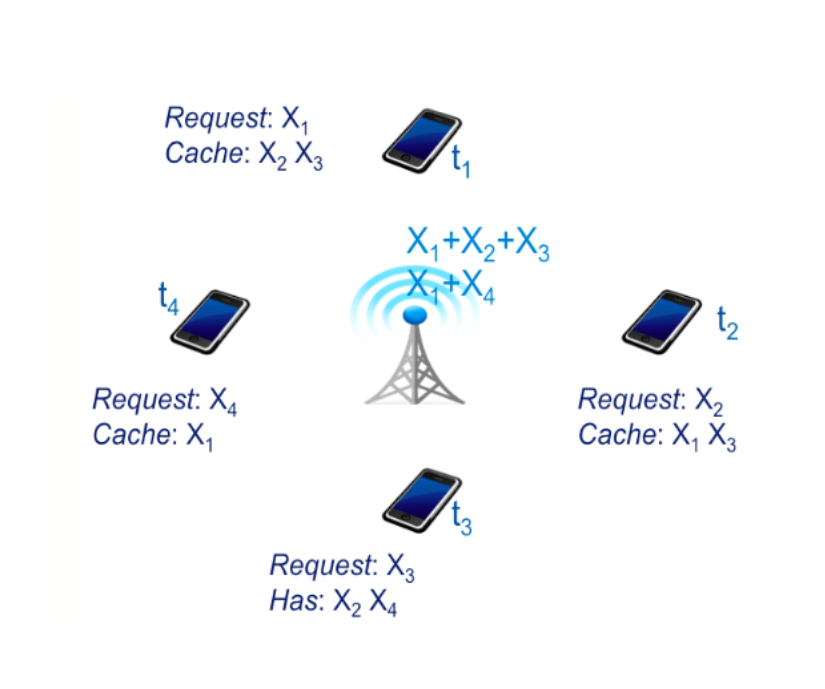
\includegraphics[width=1\linewidth]{img/p02_example1}
				%				\caption{1 server \& 4 clients}
				\label{fig:p02example1}
			\end{figure}
		}
	\end{columns}
	
\end{frame}

\section{Problem Formulation}
\subsection{PICOD Formal Defination}
\begin{frame}{PICOD Defination}
	
	\begin{columns}[c] % The "c" option specifies centered vertical alignment while the "t" option is used for top vertical alignment
		\column{.6\textwidth}
		\begin{itemize}
			\item<1-> n clients
			\item<2-> m messages $X = (X_1, \ldots, X_m)$
			\item<3-> Client $i$ knows varibles with indeices in $S_i$: $X[S_1] = \set{B_1, B_2}$
		\end{itemize}
		\column{.5\textwidth}
		
		\begin{tikzpicture}[->, >=stealth, auto, semithick]
			% Set the positions of the nodes
			\alt<1->{
				\node[circle, draw=blue, fill=blue!20] (C1) at (0,2) {$C_1$};
				\node[circle, draw=blue, fill=blue!20] (C2) at (1.5,2) {$C_2$};
				\node[circle, draw=blue, fill=blue!20] (C3) at (3,2) {$C_3$};
				\node[above] at (1.5,2.5) {clients};
			}{}
			\alt<2->{
				\node[circle, draw=green, fill=green!20] (B1) at (0,0) {$B_1$};
				\node[circle, draw=green, fill=green!20] (B2) at (1.5,0) {$B_2$};
				\node[circle, draw=green, fill=green!20] (B3) at (3,0) {$B_3$};
				\node[below] at (1.5,-0.5) {messages};
			}{}
			\alt<3->{
				% Draw the edges
				\draw (C1) -- (B2);
				\draw (C1) -- (B1);
				\draw (C2) -- (B2);
				\draw (C3) -- (B3);
			}{}
			% Position the parts
%			\begin{scope}[on background layer]
%				\alt<1->{\node[fit=(C1) (C2) (C3), draw=blue, fill=blue!10, rounded corners] {};}{}
%				\alt<2->{\node[fit=(B1) (B2) (B3), draw=green, fill=green!10, rounded corners] {};}{}
%			\end{scope}
		\end{tikzpicture}
	\end{columns}
\end{frame}
\begin{frame}{PICOD Example}
	\begin{columns}[c] % The "c" option specifies centered vertical alignment while the "t" option is used for top vertical alignment
		
		\column{.4\textwidth} 
		\begin{enumerate}[]
			
			
			\item<1->[]
			\begin{figure}
				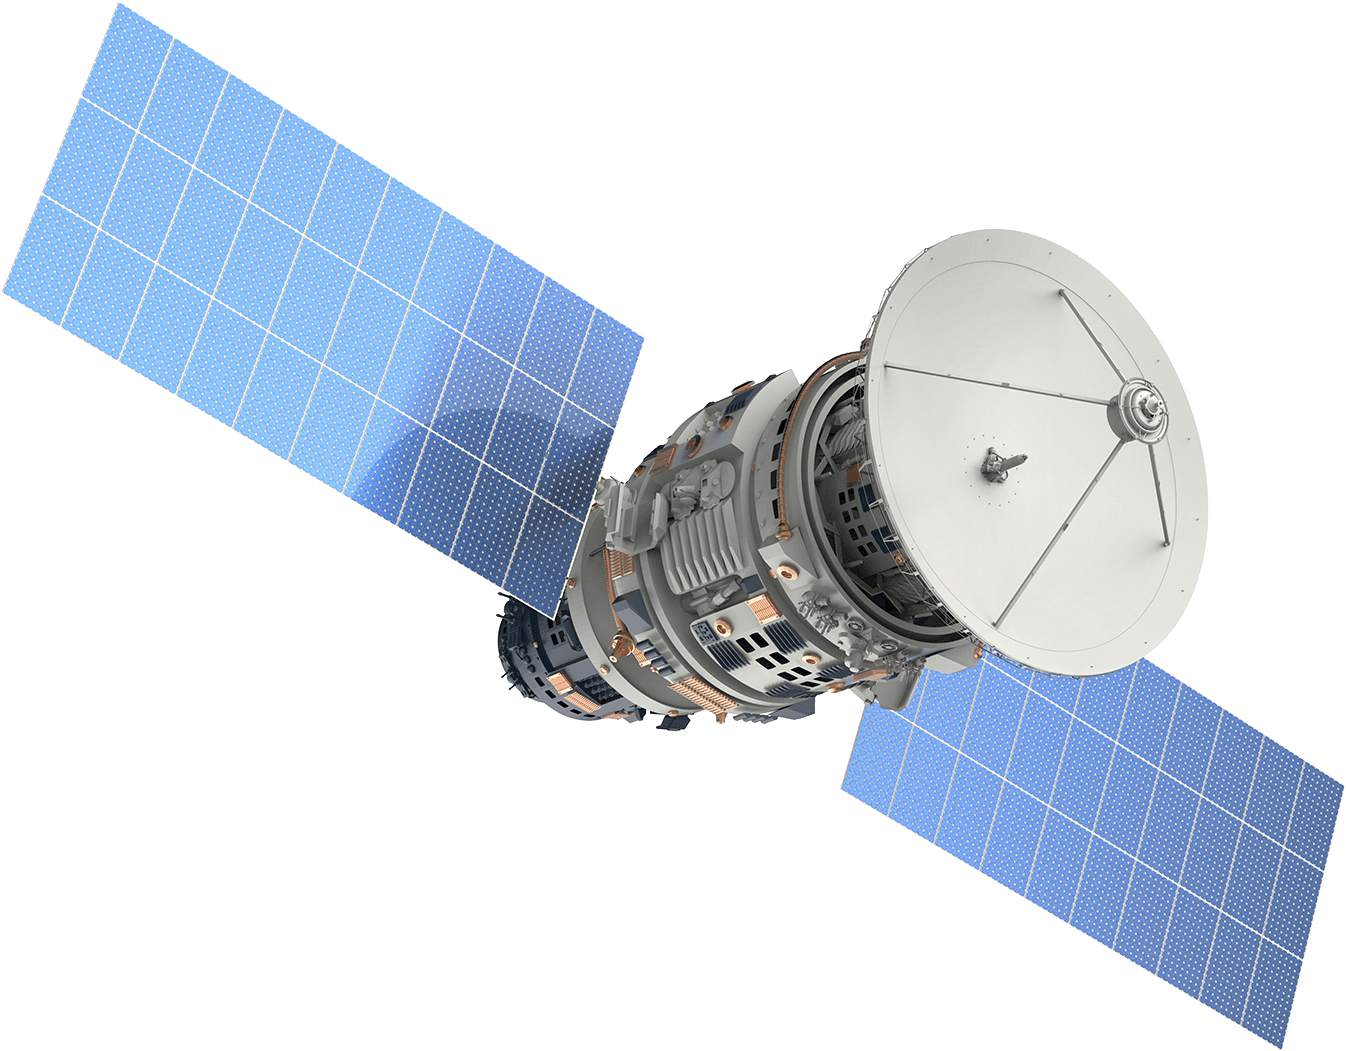
\includegraphics[width=0.4\linewidth]{img/satelite}
			\end{figure}
			
			\item<2-4>[]\centering $X_1$
			\item<3-4>[] \centering$X_2$
			\item<4-4>[] \centering$X_3$
			\item<6->[] $Y = X_1 + X_2 + X_3 $
			\item<7->[] 
			$	\begin{cases}
				X_1 &= Y - X_2 - X_3 \\
				X_2 &= Y - X_1 - X_3  \\
				X_3 &= Y - X_1 - X_2  
			\end{cases}    $
			
		\end{enumerate}
		\column{.6\textwidth} 
		\centering
		\begin{tikzpicture}[->, >=stealth, auto, semithick]
			% Set the positions of the nodes
			
			\node[circle, draw=blue, fill=blue!20, inner sep=0pt] (C1) at (0,2) {
				\alt<1-2,5>{
					
\includegraphics[width=0.06\linewidth]{img/thinkingemoji}
				}{
					
\includegraphics[width=0.06\linewidth]{img/slauthing2}
				}
			};
			\node[circle, draw=blue, fill=blue!20, inner sep=0pt] (C2) at (1.5,2) {
				\alt<4,6->{
					
\includegraphics[width=0.06\linewidth]{img/slauthing2}
				}{
					
\includegraphics[width=0.06\linewidth]{img/thinkingemoji}
				}
			};
			\node[circle, draw=blue, fill=blue!20, inner sep=0pt] (C3) at (3,2) {
				\alt<1,5>{
					
\includegraphics[width=0.06\linewidth]{img/thinkingemoji}
				}{
					
\includegraphics[width=0.06\linewidth]{img/slauthing2}
				}
			};
			\node[above] at (1.5,2.5) {We want to know more};
			
			\alt<1->{
				\node[circle, draw=green, fill=green!20, inner sep=0pt] (B1) at (0,0) {$B_1$};
				\node[circle, draw=green, fill=green!20, inner sep=0pt] (B2) at (1.5,0) {$B_2$};
				\node[circle, draw=green, fill=green!20, inner sep=0pt] (B3) at (3,0) {$B_3$};
				\node[below] at (1.5,-0.5) {messages};
			}{}
			\alt<1->{
				% Draw the edges
				\draw (C1) -- (B1);
				\alt<1-2,5>{}{\draw[->, color=red]  (C1) -- (B2);}
				\draw (C1) -- (B3);
				
				\draw (C2) -- (B1);
				\draw (C2) -- (B2);
				\alt<1-3,5>{}{\draw[->, color=red]  (C2) -- (B3);}
				
				\alt<1,5>{}{\draw[->, color=red]  (C3) -- (B1);}
				\draw (C3) -- (B2);
				\draw (C3) -- (B3);
			}{}
			% Position the parts
%			\begin{scope}[on background layer]
%				\alt<1->{\node[fit=(C1) (C2) (C3), draw=blue, fill=blue!10, rounded corners] {};}{}
%				\alt<1->{\node[fit=(B1) (B2) (B3), draw=green, fill=green!10, rounded corners] {};}{}
%			\end{scope}
		\end{tikzpicture}			
	\end{columns}
\end{frame}

\begin{frame}{ICOD vs PICOD}

	\begin{itemize}
			\item<1->[]	Similarities: 
			\begin{itemize}
				\item <2->[]
				tool: broadcast
				\item<3->[]
				clients' data: side info
			\end{itemize}
			\item<4->[]	Difference: 
			\begin{itemize}
				\item <5->[]
				Objective: clients' requirement
			\end{itemize}
		\end{itemize}
	\end{frame}
	\begin{frame}{ICOD vs PICOD. cont.}
		\begin{columns}
		\column{.5\textwidth}
		\centering
		\begin{tikzpicture}[->, >=stealth, auto, semithick]
			% Set the positions of the nodes

			\node[circle, draw=blue, fill=blue!20, inner sep=0pt] (C1) at (0,2) {
				
\includegraphics[width=0.06\linewidth]{img/thinkingemoji}
			};
			\node[circle, draw=blue, fill=blue!20, inner sep=0pt] (C2) at (1.5,2) {
				
\includegraphics[width=0.06\linewidth]{img/thinkingemoji}

			};
			\node[circle, draw=blue, fill=blue!20, inner sep=0pt] (C3) at (3,2) {
				
\includegraphics[width=0.06\linewidth]{img/thinkingemoji}
			};

			\alt<1->{
				\node[circle, draw=green, fill=green!20, inner sep=0pt] (B1) at (0,0) {$B_1$};
				\node[circle, draw=green, fill=green!20, inner sep=0pt] (B2) at (1.5,0) {$B_2$};
				\node[circle, draw=green, fill=green!20, inner sep=0pt] (B3) at (3,0) {$B_3$};
				\node[below] at (1.5,-0.5) {PICOD};
			}{}
			% Position the parts
			%			\begin{scope}[on background layer]
			%				\alt<1->{\node[fit=(C1) (C2) (C3), draw=blue, fill=blue!10, rounded corners] {};}{}
			%				\alt<1->{\node[fit=(B1) (B2) (B3), draw=green, fill=green!10, rounded corners] {};}{}
			%			\end{scope}
		\end{tikzpicture}
	\column{.5\textwidth} 
	\centering
		\begin{tikzpicture}[->, >=stealth, auto, semithick]
			% Set the positions of the nodes

			\node[circle, draw=blue, fill=blue!20, inner sep=0pt] (C1) at (0,2) {
				
\includegraphics[width=0.06\linewidth]{img/thinkingemoji}
			};
			\node[circle, draw=blue, fill=blue!20, inner sep=0pt] (C2) at (1.5,2) {
				
\includegraphics[width=0.06\linewidth]{img/thinkingemoji}

			};
			\node[circle, draw=blue, fill=blue!20, inner sep=0pt] (C3) at (3,2) {
				
\includegraphics[width=0.06\linewidth]{img/thinkingemoji}
			};

			\alt<1->{
				\node[circle, draw=green, fill=green!20, inner sep=0pt] (B1) at (0,0) {$B_1$};
				\node[circle, draw=green, fill=green!20, inner sep=0pt] (B2) at (1.5,0) {$B_2$};
				\node[circle, draw=green, fill=green!20, inner sep=0pt] (B3) at (3,0) {$B_3$};
				\node[below] at (1.5,-0.5) {ICOD};
			}{}
			\alt<1->{
			% Draw the edges
				\draw[->, color=Red]  (C1) -- (B1);


				\draw[->, color=Red]  (C2) -- (B2);

				\draw[->, color=Red]  (C3) -- (B3);
			}{}
			% Position the parts
			%			\begin{scope}[on background layer]
			%				\alt<1->{\node[fit=(C1) (C2) (C3), draw=blue, fill=blue!10, rounded corners] {};}{}
			%				\alt<1->{\node[fit=(B1) (B2) (B3), draw=green, fill=green!10, rounded corners] {};}{}
			%			\end{scope}
		\end{tikzpicture}

		\end{columns}
\end{frame}
\subsection{PICOD Algorithms}
\begin{frame}{PICOD Algorithms}
	\begin{enumerate}
	\item <1->[]
	ICOD upper bound: $n$
	\item <2->[]
	PICOD upper bound: $\log(n)$
	\item <3->[]
	PICOD algorithms: GrCov, RandCov, BinGreedy
	\end{enumerate}
\end{frame}
\subsection{Source Coding}
\begin{frame}{RDSS: Recoverable Distributed Storage System}
	\begin{figure}
		\centering
		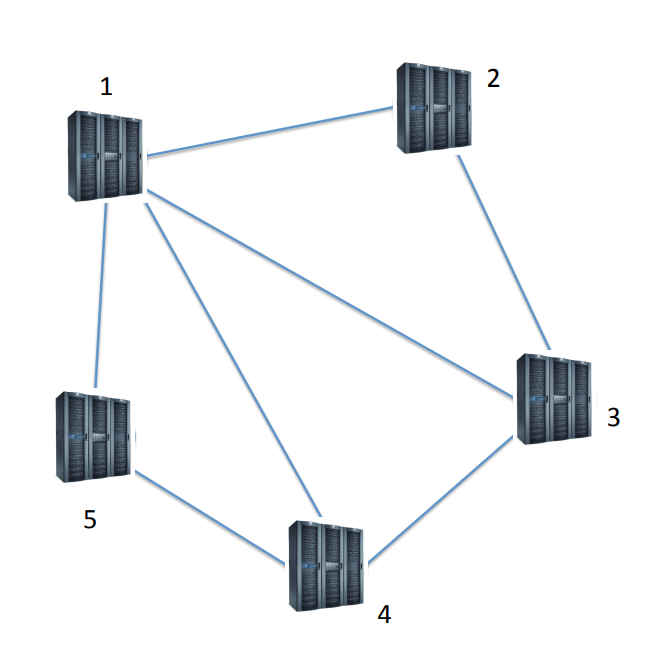
\includegraphics[width=0.5\linewidth]{img/aryaaa}
		\label{fig:aryaaa}
	\end{figure}
	
\end{frame}
\begin{frame}{Feasible Table }
	\begin{enumerate}[]
		\item<1->[]
		\begin{definition}[Feasible Table]
			For side information graph: $G$, $T \subseteq \mathbb{F}_q^m$ is a feasible table if:
			\begin{align*}
				\forall C_i: \exists j \notin S_i: \forall X, X^\prime: X[S_i] = {X^\prime}[S_i]  \Rightarrow X[j] = {X^\prime}[j]
			\end{align*}
		\end{definition}
			\end{enumerate}
	\end{frame}
	\begin{frame}{Feasible Table. cont. }
		\begin{enumerate}[]
		\item<1->[]
		\begin{example}
			\begin{columns}[c] % The "c" option specifies centered vertical alignment while the "t" option is used for top vertical alignment
				\begin{column}{.5\textwidth}
				\centering
				\begin{enumerate}
					\item<1->[] Consider side-information graph $G$.
					\item<2->[] $T_1$ is not a feasible graph because $C_3$ confuses between messages.
					\item<3->[] $T_2$ is a feasible table.
				\end{enumerate}
				\end{column}
				\begin{column}{.5\textwidth}
				\centering
				\begin{tikzpicture}[->, >=stealth, auto, semithick]
					% Set the positions of the nodes
					\node[circle, draw=blue, fill=blue!20, inner sep=0pt] (C1) at (0,2) {$C_1$};

					\node[circle, draw=blue, fill=blue!20, inner sep=0pt] (C2) at (1.5,2) {					$C_2$				};
					\node[circle, draw=blue, fill=blue!20, inner sep=0pt] (C3) at (3,2) {$C_3$				};

					\node[circle, draw=green, fill=green!20, inner sep=0pt] (B1) at (0,0) {$B_1$};
					\node[circle, draw=green, fill=green!20, inner sep=0pt] (B2) at (1.5,0) {$B_2$};
					\node[circle, draw=green, fill=green!20, inner sep=0pt] (B3) at (3,0) {$B_3$};

					\alt<1->{
					% Draw the edges
						\draw (C1) -- (B2);
						\draw (C1) -- (B3);

						\draw (C2) -- (B1);
						\draw (C2) -- (B3);



						\draw (C3) -- (B1);
						\draw (C3) -- (B2);
					}{}
					% Position the parts
%					\begin{scope}[on background layer]
%						\alt<1->{\node[fit=(C1) (C2) (C3), draw=blue, fill=blue!10, rounded corners] {};}{}
%						\alt<1->{\node[fit=(B1) (B2) (B3), draw=green, fill=green!10, rounded corners] {};}{}
%					\end{scope}
				\end{tikzpicture}
\\
				\centering
						\begin{table}[h]
					\begin{subtable}[h]{0.45\textwidth}
								\centering
							\begin{tabular}{|c|}
								\hline
								000 \\
								\hline
								001 \\
								\hline
							\end{tabular}
							\caption*{$T_1$}
						\end{subtable}
						\begin{subtable}[h]{0.45\textwidth}
							\centering
							\begin{tabular}{|c|}
								\hline
								000  \\
								011   \\
								110  \\
								101   \\
								\hline
							\end{tabular}
							\caption*{$T_2$}
						\end{subtable}
						\end{table}
				\end{column}
			\end{columns}
		\end{example}
	\end{enumerate}
\end{frame}

\begin{frame}{ Co-sets }
	\begin{enumerate}[]
		\item<1->[]
		\begin{definition}[Co-sets]
					 For sub-space $V \subseteq \mathbb{F}_q^m$, $W$ is co-set of $V$ if $\exists b\in\mathbb{F}_q^m: W = V + b$.
		\end{definition}
		\item<2->[]
		\begin{example}
			\begin{columns}
				\column{.5\textwidth}
				\begin{table}
					\begin{tabular}{|c|}
						\hline
						000 \\
						011   \\
						110  \\
						101   \\
						\hline
					\end{tabular}
					\caption*{$T_1$}
				\end{table}
				\column{.5\textwidth}
				\begin{table}
					\begin{tabular}{|c|}
						\hline
						001 \\
						010  \\
						100 \\
						111  \\
						\hline
					\end{tabular}
					\caption*{$T_2 = T_1 + (001)$}
				\end{table}
			\end{columns}
		\end{example}
	\end{enumerate}
\end{frame}


\begin{frame}{Feasible Table \& Co-sets: Example 2}
	\begin{columns}[c] % The "c" option specifies centered vertical alignment while the "t" option is used for top vertical alignment
		\column{.5\textwidth}
		\begin{enumerate}

			\item<1->[] Let's $X = (011)$
			\item <2->[] $C_1$ should guess between ${(111), (011)}$
			\item<3->[] Transmitting table label is sufficient!
		\end{enumerate}
		\column{.5\textwidth}
		\centering
		\begin{tikzpicture}[->, >=stealth, auto, semithick]
			% Set the positions of the nodes
			\node[circle, draw=blue, fill=blue!20, inner sep=0pt] (C1) at (0,2) {$C_1$};

			\node[circle, draw=blue, fill=blue!20, inner sep=0pt] (C2) at (1.5,2) {					$C_2$				};
			\node[circle, draw=blue, fill=blue!20, inner sep=0pt] (C3) at (3,2) {$C_3$				};

			\node[circle, draw=green, fill=green!20, inner sep=0pt] (B1) at (0,0) {$B_1$};
			\node[circle, draw=green, fill=green!20, inner sep=0pt] (B2) at (1.5,0) {$B_2$};
			\node[circle, draw=green, fill=green!20, inner sep=0pt] (B3) at (3,0) {$B_3$};
			\node[below] at (1.5,-0.5) {messages};

			\alt<1->{
			% Draw the edges
				\draw (C1) -- (B2);
				\draw (C1) -- (B3);

				\draw (C2) -- (B1);
				\draw (C2) -- (B3);



				\draw (C3) -- (B1);
				\draw (C3) -- (B2);
			}{}
			% Position the parts
%			\begin{scope}[on background layer]
%				\alt<1->{\node[fit=(C1) (C2) (C3), draw=blue, fill=blue!10, rounded corners] {};}{}
%				\alt<1->{\node[fit=(B1) (B2) (B3), draw=green, fill=green!10, rounded corners] {};}{}
%			\end{scope}
		\end{tikzpicture}

		\begin{columns}[c] % The "c" option specifies centered vertical alignment while the "t" option is used for top vertical alignment
			\column{.5\textwidth}
			\centering
			\begin{table}
				\begin{tabular}{|c|}
					\hline
					000 \\
					011   \\
					110  \\
					101   \\
					\hline
				\end{tabular}
				\caption*{$T_1$}
			\end{table}
			\column{.5\textwidth}
			\begin{table}
				\begin{tabular}{|c|}
					\hline
					001 \\
					010  \\
					100 \\
					111  \\
					\hline
				\end{tabular}
				\caption*{$T_2 = T_1 + (001)$}
			\end{table}
		\end{columns}
	\end{columns}
\end{frame}


\begin{frame}{Source Coding }
	\begin{enumerate}[]
		\item<1->[]
		\begin{definition}[Source coding]
			The pliable source index coding problem, PSIC, is to find the largest possible feasible table for a given $G$.
		\end{definition}
		\item<2->[]
		\begin{remark}
			\begin{itemize}[label=\Roman*.]
				\item<2->[] There is always at least one linear feasible table, $\set{\overrightarrow{0}}$.
				\item<3->[] $\mathbb{F}^n$ can be partitioned with a linear feasible table and its co-sets.
			\end{itemize}
		\end{remark}
	\end{enumerate}
\end{frame}
\begin{frame}{PICOD vs SICOD}
	\begin{itemize}
	\item<1->[]	Similarities: 
	\begin{itemize}
		\item <2->[]
				Objective: clients' requirement
		\item<3->[]
		clients' data: side info
	\end{itemize}
	\item<4->[]	Difference: 
	\begin{itemize}
		\item <5->[]
		tool: min broadcast vs max code-book
	\end{itemize}
\end{itemize}
\end{frame}
%------------------------------------------------

%------------------------------------------------
\section{Main Result}
\begin{frame}
	\centering
	\Huge
	Main Result
\end{frame}


\subsection{Main Theorem: Duality of LPICOD \& LPSCOD}
\begin{frame}{Main Theorem: Informal}
	\begin{theorem}[Duality of LPICOD \& LPSCOD]
		\begin{enumerate}
			\item <1->[]LPICOD \& LPSCOD are dual!
			\item<2->[]
			LPICOD $\Rightarrow$ LPSCOD: If you can cover all $\mathbb{F}^n$ with $r$ different sets with good properties then a feasible table with size $\lceil \dfrac{q^n}{r}\rceil $ exists.
			\item<3->[]
			LPICOD $\Leftarrow$ LPSCOD:	If a feasible table with size $|W|$ exists we can cover $\mathbb{F}^n$ with $\dfrac{q^n}{\log(|W|)}$ sets.
		\end{enumerate}
	\end{theorem}
\end{frame}
\begin{frame}{Main Theorem: Formal}
	\begin{theorem}[Duality of LPICOD \& LPSCOD]
		For any side information graph $G$, LPSICOD $(W, J, \overrightarrow{g})$ is linear algebraic dual of LPICOD $(En, I, \overrightarrow{f})$ in the sense that:
		%     \begin{enumerate}[label=\Roman*.]
			%     \item $W = ker(En)$
			%     \item    $I = J $
			%     \item    $\overrightarrow{g}_i(En(X[S_i])) = \overrightarrow{f}_i(\overrightarrow{0}, En(X[S_i])$
			%     \item $span(En) = W^{\bot} $
			%      \item $J = I$ 
			%   \item $\overrightarrow{f}_i(\overrightarrow{R}, En(X[S_i]) = g(En(X[S_i] - R[S_i])) + R[I_i]$ where $ \exists! V \in W: V + R = X $
			% \end{enumerate}
		\begin{align*}
			(W, J, \overrightarrow{g}) &= \begin{cases}
				W = ker(En)\\
				I = J \\    
				\overrightarrow{g}_i(En(X[S_i])) = \overrightarrow{f}_i(\overrightarrow{0}, En(X[S_i])\\
			\end{cases} \\
			(En, I, \overrightarrow{f}) &= \begin{cases}
				span(En) = W^{\bot} \\
				J = I \\
				\overrightarrow{f}_i(\overrightarrow{R}, En(X[S_i]) =\\ g(En(X[S_i] - R[S_i])) + R[I_i]: \exists! V \in W: V + R = X \\
			\end{cases}
		\end{align*}
		% $span(En) = W^{\bot},
		% W = ker(En), I = J,
		% \overrightarrow{g}_i(En(X[S_i])) = \overrightarrow{f}_i(\overrightarrow{0}, En(X[S_i]),
		% \overrightarrow{f}_i(\overrightarrow{R}, En(X[S_i]) = g(En(X[S_i] - R[S_i])) + R[I_i]
		% $ where $\exists! V \in W: V + R = X $ 
		$dim(W) = n - dim(En)$
	\end{theorem}
\end{frame}


\begin{frame}{Main Theorem: Proof Ideas}
	\begin{itemize}
		\item<1-> $PLICOD \Rightarrow PLSCOD$, easy direction: messages with encoded code $\overrightarrow{0}$ form a feasible table
		
		\item<2-> $PLSCOD \Rightarrow PLICOD$, hard direction: feasible table and its co-sets partition $\mathbb{F}^n$
	\end{itemize}
\end{frame}
\subsection{Hard Example}
\begin{frame}{Hard Example}
	\begin{itemize}
		\item<1->[]
			\begin{example}
				\begin{itemize}
					\item<1->[] PICOD with side information from a sub-space
					\item<2->[] $V_1, \ldots, V_n$ a basis of V
					\item<3->[] $C_i = V_i$
					\item<4->[] Using extended version of Mazumdar's inequality for PICOD we show there exists a haard example needing $\log(n)$ even for non-linear codes
				\end{itemize}
			\end{example}
		\item <5->[]
			\begin{theorem}[Mazumdar]
				\begin{align*}
					n - \rdss_q(G) \le \indx_q(G) &\le n -\rdss_q(G) \\
					&+ \log_q\Big(\min\set{n\ln q, 1+ \rdss_q(G)\ln q }\Big)
				\end{align*}
			\end{theorem}
	\end{itemize}
\end{frame}
\subsection{Future Work}
\begin{frame}{Future Work}
	\begin{itemize}
		\item<1-> Similar work for the very pliable problem
		\item<2-> Tighter bounds for the non-linear case
		\item<3-> Better shifts and covers
		\item<4-> content type coding
		
	\end{itemize}
\end{frame}

%------------------------------------------------



\begin{frame}{refrences}
	%		\bibliographystyle{plain}
	\printbibliography
	
	%\bibliographystyle{ieeetr} % We choose the "plain" reference style
	%	\bibliography{refs} % Entries are in the refs.bib file
\end{frame}
\setbeamertemplate{footline}{}
\begin{frame}
    \centering
    \vspace{1cm}
    \hspace{2cm} \smaller{In} \textbf{\Huge{THE END}} \smaller{it doesn't even matter}\\
    \vspace{0.5cm}
    \textit{\Large{Thank you for your attention}}
\end{frame}


\begin{frame}{GrCov}
	\begin{definition}
		$\forall B_1 \subseteq B: W_i(B_1) := \card{\set{c_j \in C: c \in N(B_1), N(c) \cap B_1 = |B_1| - i }}$
	\end{definition}
	\begin{lemma}
		For $d_{max} = \max\set{R_i}, d_{min} = \min\set{R_i}$, if there exists a constant $r$ such that $d_{max} \leq r d_{min}$ then there exists a code with lenght $O(\log(n))$
	\end{lemma}
	\begin{theorem}
		For a $(n, m)$ PICOD there exists a code with lenght:
			$$O(\min\set{m, n, \log(m)(1 + \log^{+}(\dfrac{n}{\log(m)}) ))})$$
	\end{theorem}
\end{frame}
\begin{frame}{BinGreedy}
			\begin{itemize}
				\item<1->[]
	\begin{definition}
		For Permutation $\pi = (j_1, \ldots, j_m)$ of messages, we define effectie degree of $b_{j_t}$ as $\card{\set{c_i: c_i \in N[]b_{j_t}], \forall t' < t: c_i \notin N[b_{j_{t'}}]}}$
	\end{definition}
	\item<2->[]
	\begin{algg}
		\begin{itemize}
			\item<2-> Sorting: in $t$-th iteration pick $j_t$ as the message node with maximum degree from from $[m] \setminus \set{j_1, \ldots, j_{t - 1}}$
			\item<3-> partition permutation in $\log(n)$ sets such that $\dfrac{n}{2^{s - 1}} \geq d^\dagger[j] > \dfrac{n}{2^s}$
			\item<4-> send a code for each set.
		\end{itemize}
	\end{algg}
			\end{itemize}
\end{frame}

\begin{frame}{BinGreedy. cont.}
	\begin{theorem}[efficency]
			\begin{itemize}
			\item<1-> code lengh is at most $\dfrac{2}{\log(1.5)} \log^2(n)$
			 \item<2-> BinGreedy runs in $O(n m^2 \log(n))$ 
			\item<3-> approximation ratio $\alpha(n)$ satiffy: 	$$\Omega(\log \log (n)) \leq \alpha(n) \leq O(\log^2(n))$$
			\end{itemize}
	\end{theorem}
\end{frame}
% \begin{frame}[allowframebreaks]
%         \frametitle{References}
%%         \bibliographystyle{ieeetr}
%         \bibliography{refs}
% \end{frame}

\end{document}